% !TeX spellcheck = en_GB
%%%%%%%%%%%%%%%%%%%%%%%%%%%%%%%%%%%%%%%%%
% Beamer Presentation
% LaTeX Template
% Version 1.0 (10/11/12)
%
% This template has been downloaded from:
% http://www.LaTeXTemplates.com
%
% License:
% CC BY-NC-SA 3.0 (http://creativecommons.org/licenses/by-nc-sa/3.0/)
%
%%%%%%%%%%%%%%%%%%%%%%%%%%%%%%%%%%%%%%%%%

%----------------------------------------------------------------------------------------
%     PACKAGES AND THEMES
%----------------------------------------------------------------------------------------
% !TeX TXS-program:compile = txs:///pdflatex/[--shell-escape]
\documentclass{beamer}
%\usepackage[ngerman]{babel}


\mode<presentation> {

% The Beamer class comes with a number of default slide themes
% which change the colors and layouts of slides. Below this is a list
% of all the themes, uncomment each in turn to see what they look like.

%\usetheme{default}
%\usetheme{AnnArbor}
%\usetheme{Antibes}
%\usetheme{Bergen}
%\usetheme{Berkeley}
%\usetheme{Berlin}
%\usetheme{Boadilla}
%\usetheme{CambridgeUS}
%\usetheme{Copenhagen}
%\usetheme{Darmstadt}
%\usetheme{Dresden}
%\usetheme{Frankfurt}
%\usetheme{Goettingen}
%\usetheme{Hannover}
%\usetheme{Ilmenau}
%\usetheme{JuanLesPins}
%\usetheme{Luebeck}
\usetheme{Madrid}
%\usetheme{Malmoe}
%\usetheme{Marburg}
%\usetheme{Montpellier}
%\usetheme{PaloAlto}
%\usetheme{Pittsburgh}
%\usetheme{Rochester}
%\usetheme{Singapore}
%\usetheme{Szeged}
%\usetheme{Warsaw}

% As well as themes, the Beamer class has a number of color themes
% for any slide theme. Uncomment each of these in turn to see how it
% changes the colors of your current slide theme.

%\usecolortheme{albatross}
%\usecolortheme{beaver}
%\usecolortheme{beetle}
%\usecolortheme{crane}
%\usecolortheme{dolphin}
%\usecolortheme{dove}
%\usecolortheme{fly}
%\usecolortheme{lily}
%\usecolortheme{orchid}
%\usecolortheme{rose}
%\usecolortheme{seagull}
%\usecolortheme{seahorse}
%\usecolortheme{whale}
%\usecolortheme{wolverine}

%\setbeamertemplate{footline} % To remove the footer line in all slides uncomment this line
%\setbeamertemplate{footline}[page number] % To replace the footer line in all slides with a simple slide count uncomment this line

%\setbeamertemplate{navigation symbols}{} % To remove the navigation symbols from the bottom of all slides uncomment this line
}

\usepackage{graphicx} % Allows including images
\usepackage{booktabs} % Allows the use of \toprule, \midrule and
% \bottomrule in tables
\usepackage{listings}
\usepackage{parcolumns}
\usepackage[nocenter]{qtree}
\usepackage{minted}
\usepackage{eurosym}
\usepackage{qrcode}
\usepackage{xcolor}
\definecolor{LightGray}{gray}{0.95}
%----------------------------------------------------------------------------------------
%     TITLE PAGE
%----------------------------------------------------------------------------------------

\title[]{Introduction to programming in Python} % The short title appears at the bottom of every slide, the full title is only on the title page

\author{Jules Kreuer} % Your name
\institute[FSI] % Your institution as it will appear on the bottom of every slide, may be shorthand to save space
{
Uni Tübingen\\ % Your institution for the title page
\medskip
\textit{fsi@fsi.uni-tuebingen.de}\\
\textit{contact@juleskreuer.eu}\\
}
\date{\today} % Date, can be changed to a custom date

\begin{document}

\begin{frame}
\titlepage % Print the title page as the first slide
\end{frame}

%----------------------------------------------------------------------------------------
%     PRESENTATION SLIDES
%----------------------------------------------------------------------------------------

\begin{frame}
	Based on:\\\\
	Ana Bell, Eric Grimson, and John Guttag. \\
	6.0001 Introduction to Computer Science and Programming in Python.\\
	Fall 2016. Massachusetts Institute of Technology: MIT OpenCourseWare\\
	https://ocw.mit.edu.\\
	License: Creative Commons BY-NC-SA.\\\\
	
	Nick Parlante, John Cox, Steve Glassman, Piotr Kaminksi, Antoine Picard.\\
	Google's Python Class.\\
	July 2015. Google LLC\\
	License: Creative Commons BY 2.5.	
\end{frame}

\begin{frame}
	\begin{block}{}<1->
		\textbf{Part 1: Hello World}\\
		- Introduction\\ 
		- Installation \\
		- REPL\\
	\end{block}
	\begin{exampleblock}{}
	Break
	\end{exampleblock}
	\begin{block}{}<2->
	\textbf{Part 2: Basics}\\
	- Common operators\\
	- Data objects / data types\\
	- Strings, input, type-casting\\
	- Lists, dicts\\
	- Control flow: for, while, break
	\end{block}
	\begin{exampleblock}{}<2->
		Break
	\end{exampleblock}
\end{frame}

\begin{frame}
	\begin{block}{}
		\textbf{Part 3: Abstraction}\\
		- Functions, variable scope, lambda\\
		- recursion\\
		- Objects, Classes\\
	\end{block}
	\begin{exampleblock}{}
	Break
	\end{exampleblock}
	\begin{block}{}<2->
		\textbf{Part 4: Development}\\
		- Arguments\\
		- Modules / imports\\
		- V-Envs
		- Tests
	\end{block}
\end{frame}

\begin{frame}[fragile]
	\frametitle{Demo}
	\begin{minted}{bash}
jules@T480:~$ python3
Python 3.8.10 (default, Nov 26 2021, 20:14:08) 
[GCC 9.3.0] on linux
Type "help", "copyright", "credits" or "license"...
	\end{minted}
\begin{minted}{python}
>>> a = 5
>>> a
5
>>> a = "Hello World"
>>> a
'Hello World'
>>> a + "!"
'Hello World!'
>>> 
	\end{minted}
\end{frame}

\begin{frame}
	\frametitle{Installation / REPL}
	\begin{center}
		\url{https://www.python.org/downloads/}\\
		Debian / Ubuntu: \textit{sudo apt install python3}\\
	\end{center}
	\begin{center}
		Type in your shell: \textit{python3}
	\end{center}
\end{frame}

\begin{frame}
	\begin{figure}
		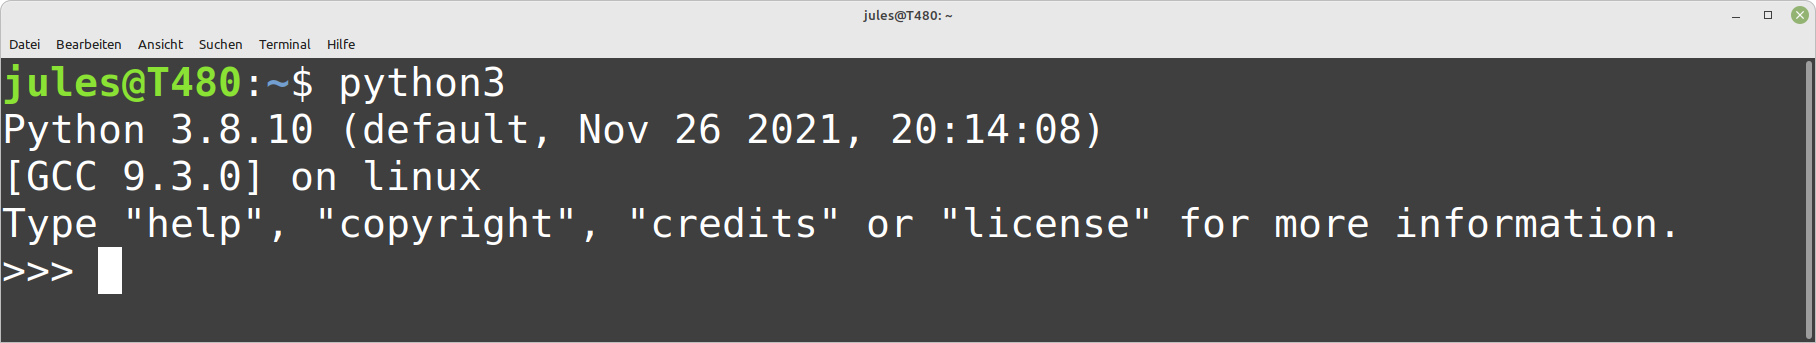
\includegraphics[width=12cm]{figures/console.png}
		\caption{Python3 REPL}
	\end{figure}
\end{frame}

\begin{frame}[fragile]
	\begin{block}{Running code}
		- REPL\\
		- python3 file args
	\end{block}
	\begin{example}
			\begin{minted}{bash}
python3 hello-world.py
		\end{minted}
	\end{example}
\end{frame}

\begin{frame}
	\frametitle{Combining Editor and Interpreter}
	\begin{figure}
		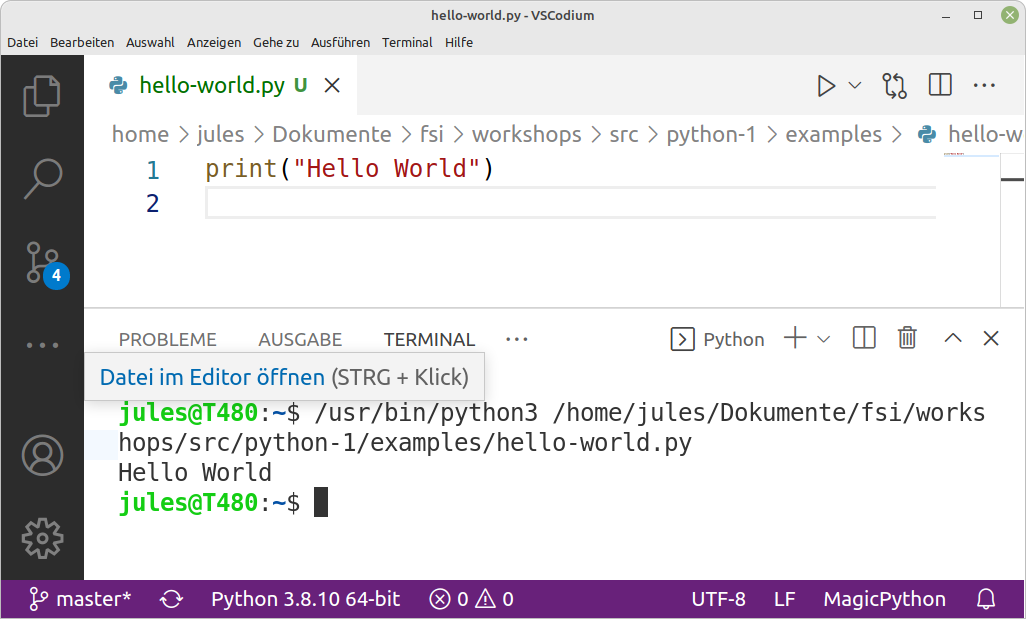
\includegraphics[width=8cm]{figures/vs-code.png}
		\caption{VS Codium}
	\end{figure}
\end{frame}
\begin{frame}
	\textbf{Possible IDEs / Editors:}\\
	- VS Codium: \url{https://vscodium.com/}\\
	- PyCharm: \url{https://www.jetbrains.com/pycharm/}\\
	- Atom: \url{https://atom.io/}\\
	- ...
\end{frame}

\begin{frame}[fragile]
	\frametitle{hello-world.py}
	- Content: \mintinline{python}{print("Hello World")}\\
	- Run it!
\end{frame}


\end{document} 